% Build from repository root:
% mkdir -p /tmp/cupami-diagram
% tectonic --outdir /tmp/cupami-diagram docs/figures/gpu-pipeline.tex
% pdftocairo -svg /tmp/cupami-diagram/gpu-pipeline.pdf docs/figures/gpu-pipeline.svg
\documentclass[tikz,border=6pt]{standalone}
\usepackage[T1]{fontenc}
\usepackage{lmodern}
\usetikzlibrary{arrows.meta}
\begin{document}
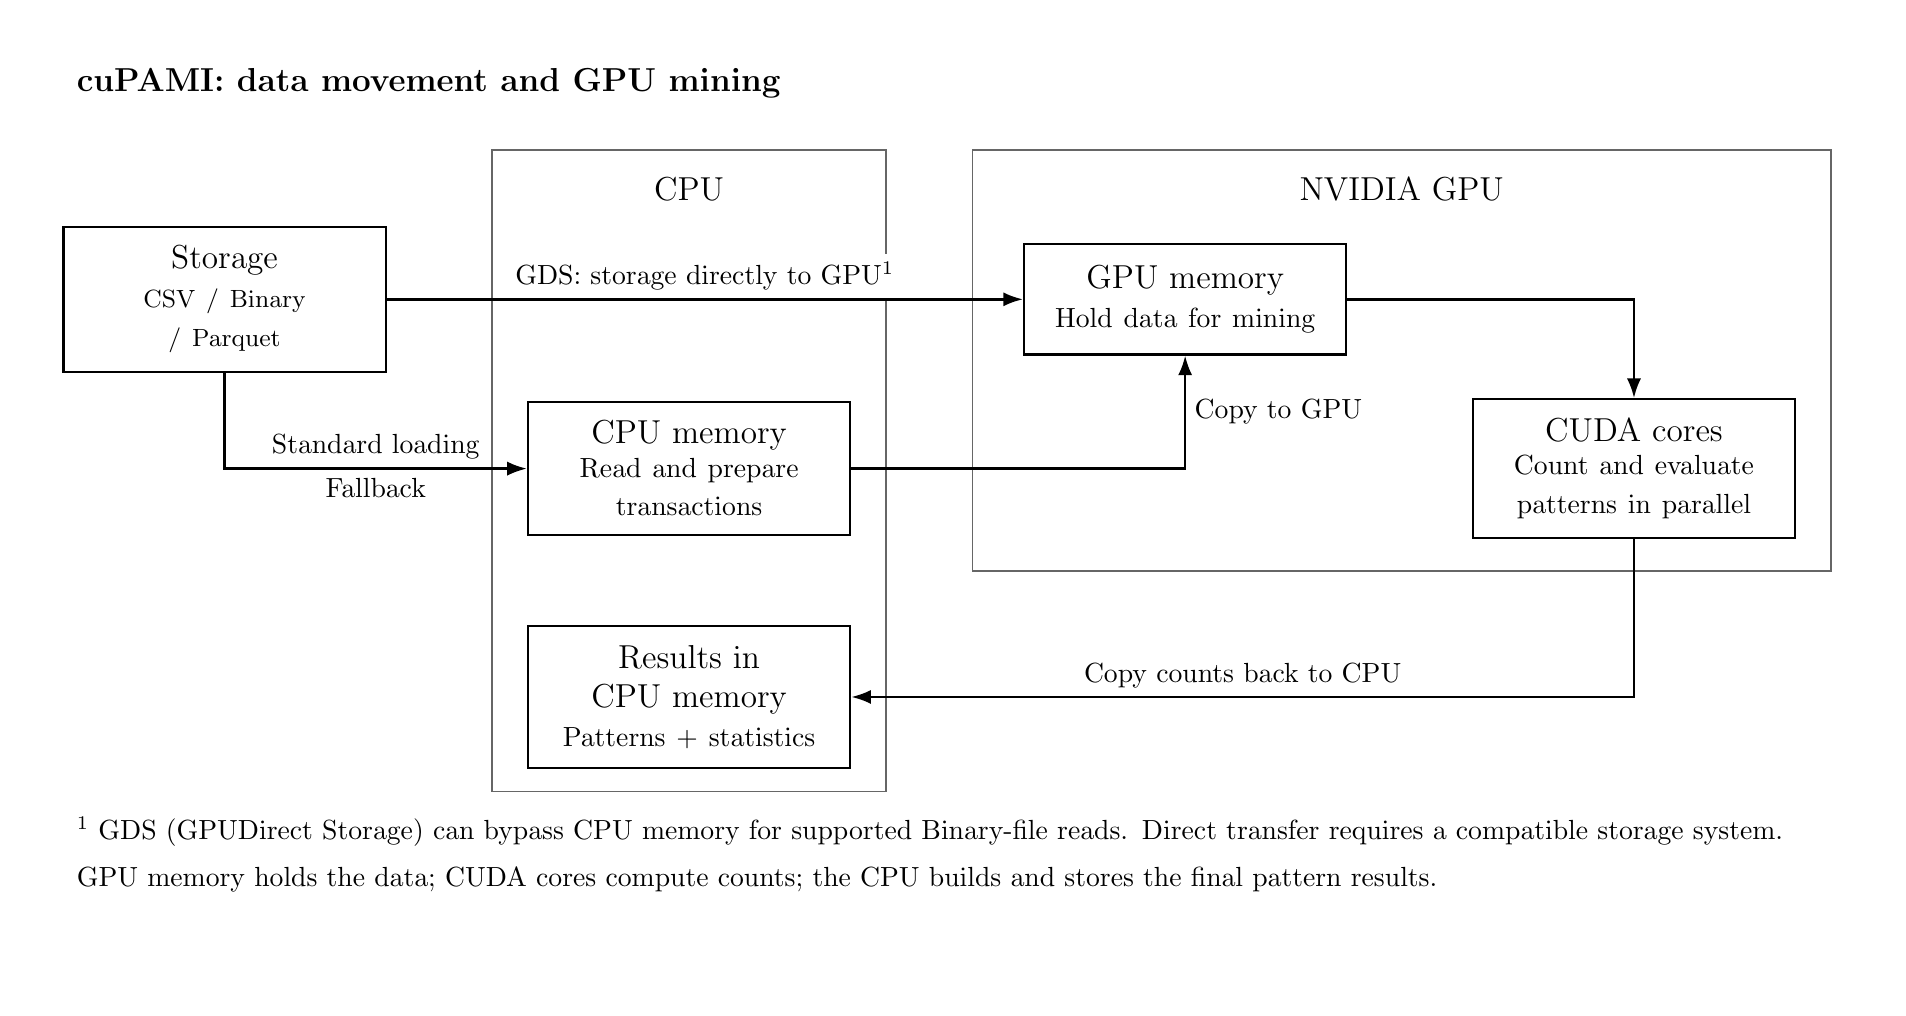
\begin{tikzpicture}[x=1cm,y=1cm,font=\large,
 box/.style={draw=black,line width=.8pt,fill=white,align=center,minimum height=1.4cm,text width=3.6cm,inner sep=7pt},
 flow/.style={-{Latex[length=2.5mm,width=1.8mm]},line width=.9pt},
 label/.style={font=\normalsize,align=center,fill=white,inner sep=3pt}]
% Opaque canvas for light and dark README themes.
\fill[white] (-.5,-4.0) rectangle (23,8.2);
\node[anchor=west,font=\large\bfseries] at (0,7.5) {cuPAMI: data movement and GPU mining};
% Host and device are physical regions, with a simple two-route input path.
\draw[black!60,line width=.6pt] (5.4,-1.5) rectangle (10.4,6.65);
\node at (7.9,6.15) {CPU};
\draw[black!60,line width=.6pt] (11.5,1.3) rectangle (22.4,6.65);
\node at (16.95,6.15) {NVIDIA GPU};
\node[box] (storage) at (2,4.75) {Storage\\\small CSV / Binary / Parquet};
\node[box] (host) at (7.9,2.6) {CPU memory\\\normalsize Read and prepare\\transactions};
\node[box] (device) at (14.2,4.75) {GPU memory\\\normalsize Hold data for mining};
\node[box] (cores) at (19.9,2.6) {CUDA cores\\\normalsize Count and evaluate\\patterns in parallel};
% GDS bypasses host data staging when supported.
\draw[flow] (storage.east) -- node[label,above] {GDS: storage directly to GPU\textsuperscript{1}} (device.west);
\draw[flow] (storage.south) -- (2,2.6) -- node[label,above] {Standard loading} node[label,below] {Fallback} (host.west);
\draw[flow] (host.east) -- (14.2,2.6) -- node[label,right] {Copy to GPU} (device.south);
\draw[flow] (device.east) -- (19.9,4.75) -- (cores.north);

% CPU directs repeated GPU operations and receives measurements.
\node[box] (results) at (7.9,-.3) {Results in CPU memory\\\normalsize Patterns + statistics};

\draw[flow] (cores.south) -- (19.9,-.3) -- node[label,above] {Copy counts back to CPU} (results.east);
\node[anchor=north west,align=left,text width=22cm,font=\normalsize] at (0,-1.7) {
\textsuperscript{1} GDS (GPUDirect Storage) can bypass CPU memory for supported Binary-file reads. Direct transfer requires a compatible storage system.\\[5pt]
GPU memory holds the data; CUDA cores compute counts; the CPU builds and stores the final pattern results.};
\end{tikzpicture}
\end{document}
